
\begin{abox}
	Practice set-1
\end{abox}
\begin{enumerate}[label=\color{ocre}\textbf{\arabic*.}]
	\item Consider the matrix $M=\left(\begin{array}{lll}1 & 1 & 1 \\ 1 & 1 & 1 \\ 1 & 1 & 1\end{array}\right)$\\
	\textbf{A.} The eigenvalues of $M$ are
	{\exyear{NET/JRF(JUNE-2011)}}
	\begin{tasks}(4)
		\task[\textbf{A.}] $0,1,2$
		\task[\textbf{B.}] $0,0,3$
		\task[\textbf{C.}] $1,1,1$
		\task[\textbf{D.}] $-1,1,3$
	\end{tasks}
	\begin{answer}
		\begin{align*}
		\text{For eigen values }\left[\begin{array}{ccc}1-\lambda & 1 & 1 \\ 1 & 1-\lambda & 1 \\ 1 & 1 & 1-\lambda\end{array}\right]&=0\\
		(1-\lambda)\left((1-\lambda)^{2}-1\right)-(1-\lambda-1)+1(1-(1-\lambda))&=0\\
		(1-\lambda)\left(1+\lambda^{2}-2 \lambda-1\right)+\lambda+\lambda=0 \Rightarrow \lambda^{2}-2 \lambda-\lambda^{3}+2 \lambda^{2}+2 \lambda&=0\\
		\lambda^{3}-3 \lambda^{2}=0 \Rightarrow \lambda^{2}(\lambda-3)=0 \Rightarrow \lambda&=0,0,3
		\intertext{For any $n \times n$ matrix having all elements unity eigenvalues are $0,0,0, \ldots, n$.}
		\end{align*}
		So the correct answer is \textbf{Option (B)}
	\end{answer}
	\textbf{B.} The exponential of $M$ simplifies to ( $I$ is the $3 \times 3$ identity matrix)
	\begin{tasks}(2)
		\task[\textbf{A.}] $e^{M}=I+\left(\frac{e^{3}-1}{3}\right) M$
		\task[\textbf{B.}] $e^{M}=I+M+\frac{M^{2}}{2 !}$
		\task[\textbf{C.}] $e^{M}=I+3^{3} M$
		\task[\textbf{D.}] $e^{M}=(e-1) M$
	\end{tasks}
	\begin{answer}
		\begin{align*}
	\intertext{We know that}
	e^x&=1+x+\frac{x^2}{2!}+\frac{x^3}{3!}+.....\\
	e^M&=1+M+\frac{M^2}{2!}+\frac{M^3}{3!}+.....\\
	M&=\left[\begin{array}{lll}1 & 1 & 1 \\ 1 & 1 & 1 \\ 1 & 1 & 1\end{array}\right] \Rightarrow M^{2} =\left[\begin{array}{lll}3 & 3 & 3 \\ 3 & 3 & 3 \\ 3 & 3 & 3\end{array}\right]=3 M\\
	\text{similarly}\quad M^{3}&=9 M=3^{2} M
	\intertext{we can rewrite $e^M$ as,}
	e^{M}&=I+M+\frac{3 M}{2 !}+\frac{3^{2} M}{3 !}+\frac{3^{3} M}{4 !}+\cdots\\
	&=I+\frac{M}{3}\left[3+\frac{3^{2}}{2 !}+\frac{3^{3}}{3 !}+\frac{3^{4}}{4 !}+\cdots\right]\\
	&=I+\frac{M}{3}\left[e^{3}-1\right]
		\end{align*}
	\end{answer}
	\item A $3 \times 3$ matrix $M$ has $\operatorname{Tr}[M]=6, \operatorname{Tr}\left[M^{2}\right]=26$ and $\operatorname{Tr}\left[M^{3}\right]=90$. Which of the following can be a possible set of eigenvalues of $M ?$
	{\exyear{NET/JRF(DEC-2011)}}
\begin{tasks}(4)
\task[\textbf{A.}] $\{1,1,4\}$
\task[\textbf{B.}] $\{-1,0,7\}$
\task[\textbf{C.}] $\{-1,3,4\}$
\task[\textbf{D.}] $\{2,2,2\}$
\end{tasks}
\begin{answer}
\begin{align*}
T_r[M]&=\text{sum of eigen values}\\
T_r[M^2]&=\text{sum of square of eigen values}\\
\operatorname{Tr}\left[M^{2}\right]&=(-1)^{2}+(3)^{2}+(4)^{2}\text{ also } \operatorname{Tr}\left[M^{3}\right]\\&=(-1)^{3}+(3)^{3}+(4)^{3}=90
\end{align*}
So the correct answer is \textbf{Option (C)}
\end{answer}
\item The eigen values of the matrix $A=\left(\begin{array}{lll}1 & 2 & 3 \\ 2 & 4 & 6 \\ 3 & 6 & 9\end{array}\right)$ are
{\exyear{NET/JRF(JUNE-2012)}}
\begin{tasks}(4)
	\task[\textbf{A.}] $(1,4,9)$
	\task[\textbf{B.}] $(0,7,7)$
	\task[\textbf{C.}] $(0,1,13)$
	\task[\textbf{D.}] $(0,0,14)$
\end{tasks}
\begin{answer}
	 
	\begin{align*}
	\intertext{The given matrix $A$ has identical rows and columns}
	\intertext{So it's eigen values are,}
	\lambda=0,0\ \text{Trace}=0,0,14
	\intertext{Another solution}
	\text{For eigenvalues }|A-\lambda I|=0 \Rightarrow\left[\begin{array}{ccc}1-\lambda & 2 & 3 \\ 2 & 4-\lambda & 6 \\ 3 & 6 & 9-\lambda\end{array}\right]&=0\\
	(1-\lambda)[(4-\lambda)(9-\lambda)-36]-2[2(9-\lambda)-18]+3[12-3(4-\lambda)]&=0\\
	(1-\lambda)(4-\lambda)(9-\lambda)-36(1-\lambda)-4(9-\lambda)+36+9 \lambda&=0\\
	\lambda^{3}-14 \lambda^{2}=0 \Rightarrow \lambda^{2}(\lambda-14)=0 \Rightarrow \lambda&=0,0,14
	\end{align*}
	So the correct answer is \textbf{Option (D)}
\end{answer}
	\item The eigenvalues of the antisymmetric matrix,
	$$
	A=\left(\begin{array}{ccc}
	0 & -n_{3} & n_{2} \\
	n_{3} & 0 & -n_{1} \\
	-n_{2} & n_{1} & 0
	\end{array}\right)
	$$
	where $n_{1}, n_{2}$ and $n_{3}$ are the components of a unit vector, are
	{\exyear{NET/JRF(JUNE-2012)}}
	\begin{tasks}(4)
		\task[\textbf{A.}] $0, i,-i$
		\task[\textbf{B.}] $0,1,-1$
		\task[\textbf{C.}] $0,1+i,-1,-i$
		\task[\textbf{D.}]  $0,0,0$
	\end{tasks}
	\begin{answer}
		\begin{align*}
		A&=\left[\begin{array}{ccc}0 & -n_{3} & n_{2} \\ n_{3} & 0 & -n_{1} \\ -n_{2} & n_{1} & 0\end{array}\right] \Rightarrow-A^{T}=\left[\begin{array}{ccc}0 & -n_{3} & n_{2} \\ n_{3} & 0 & -n_{1} \\ -n_{2} & n_{1} & 0\end{array}\right]\\
		(A-\lambda I)&=0,\left[\begin{array}{ccc}0-\lambda & -n_{3} & n_{2} \\ n_{3} & 0-\lambda & -n_{1} \\ -n_{2} & n_{1} & 0-\lambda\end{array}\right]=0\\
		\Rightarrow \lambda_{1}&=0 \Rightarrow \lambda_{2}=-\sqrt{-n_{1}^{2}-n_{2}^{2}-n_{3}^{2}} \Rightarrow \lambda_{3}\\&=\sqrt{-n_{1}^{2}-n_{2}^{2}-n_{3}^{2}}\\
		\text{but }&\sqrt{n_{1}^{2}+n_{2}^{2}+n_{3}^{2}}=1\\
		\intertext{For an antisymmetric matrix the eigen values are}
		\lambda &=0,\pm i
		\intertext{sum of sqares of non diagonal elements}
		&=0,\pm i \sqrt{n_1^2+n_2^2+n_3^2}=0, \pm i\\
		\therefore &n_1, n_2, n_3 \text{are components of a unit vector}\\
		\text{	so, }\quad \lambda_{1}&=0, \lambda_{2}=i, \lambda_{3}=-i\\
		A&=-A^{T}\text{ (Antisymmetric). Eigenvalues are either zero or purely imaginary.}
		\end{align*}
		So the correct answer is \textbf{Option (A)}
	\end{answer}
	\item Consider an $n \times n(n>1)$ matrix $A$, in which $A_{i j}$ is the product of the indices $i$ and $j$ $\left(\right.$ namely $\left.A_{i j}=i j\right)$. The matrix $A$
{\exyear{NET/JRF(DEC-2013)}}
	\begin{tasks}(1)
		\task[\textbf{A.}]  Has one degenerate eigevalue with degeneracy $(n-1)$
		\task[\textbf{B.}] Has two degenerate eigenvalues with degeneracies 2 and $(n-2)$
		\task[\textbf{C.}] Has one degenerate eigenvalue with degeneracy $n$
		\task[\textbf{D.}] Does not have any degenerate eigenvalue
	\end{tasks}
	\begin{answer}
	\begin{align*}
	\intertext{The matrix $A$ will be like, }
	A_{i j}=\left[\begin{array}{ccccccc}1 & 2 & 3 & 4 & \cdots & n \\ 2 & 4 & 6 & 8 & \cdots & \cdots & \\ 3 & 6 & 9 & 12 & \cdots & \cdots \\ 4 & 8 & 12 & 16 & \cdots & \cdots \\ \vdots & \vdots & \vdots & \vdots & \vdots & \vdots \\ n & \vdots & \vdots & \vdots & & \end{array}\right]
	\intertext{The matrix $A$ is having identical rows and columns then it's eigen values will be, $(n-1)$ number of zeros and it's trace.}
	\lambda&=0,0,.......,[1^2+2^2+....n^2]
	\intertext{Thus the matrix has one degenerate eigen value with $n-1$  degeneracy}
	\end{align*}
		So the correct answer is \textbf{Option (A)}
	\end{answer}
	\item Consider the matrix
	$$
	M=\left(\begin{array}{ccc}
	0 & 2 i & 3 i \\
	-2 i & 0 & 6 i \\
	-3 i & -6 i & 0
	\end{array}\right)
	$$
	The eigenvalues of $M$ are
	{\exyear{NET/JRF(JUNE-2014)}}
	\begin{tasks}(4)
		\task[\textbf{A.}] $-5,-2,7$
		\task[\textbf{B.}] $-7,0,7$
		\task[\textbf{C.}] $-4 i, 2 i, 2 i$
		\task[\textbf{D.}] $2,3,6$
	\end{tasks}
	\begin{answer}
		\begin{align*}
		M&=\left(\begin{array}{ccc}0 & 2 i & 3 i \\ -2 i & 0 & 6 i \\ -3 i & -6 i & 0\end{array}\right), M^{+}=\left(\begin{array}{ccc}0 & 2 i & 3 i \\ -2 i & 0 & 6 i \\ -3 i & -6 i & 0\end{array}\right)\\
		M^{+}&=M
		\intertext{Matrix is Hermitian so roots are real and }
		\lambda&=0,\pm i\sqrt{(2i)^2+(3i)^2+(6i)^2}\quad\text{property of antisymmetric matrix}\\
		&=0,\pm i\sqrt{-49}\\
		&=0,\pm 7=-7,0,7
		\end{align*}
		So the correct answer is \textbf{Option (B)}
	\end{answer}
	\item The column vector $\left(\begin{array}{l}a \\ b \\ a\end{array}\right)$ is a simultaneous eigenvector of $A=\left(\begin{array}{ccc}0 & 0 & 1 \\ 0 & 1 & 0 \\ 1 & 0 & 0\end{array}\right)$ and $B=\left(\begin{array}{lll}0 & 1 & 1 \\ 1 & 0 & 1 \\ 1 & 1 & 0\end{array}\right)$ if
	{\exyear{NET/JRF(DEC-2014)}}
	\begin{tasks}(2)
		\task[\textbf{A.}] $b=0$ or $a=0$
		\task[\textbf{B.}] $b=a$ or $b=-2 a$
		\task[\textbf{C.}] $b=2 a$ or $b=-a$
		\task[\textbf{D.}] $b=a / 2$ or $b=-a / 2$
	\end{tasks}
	\begin{answer}
		\begin{align*}
		\text{Let }b&=a\\
		\left(\begin{array}{lll}0 & 0 & 1 \\ 0 & 1 & 0 \\ 1 & 0 & 0\end{array}\right)\left(\begin{array}{l}a \\ a \\ a\end{array}\right)&=\left(\begin{array}{l}a \\ a \\ a\end{array}\right)\text{ and } \left(\begin{array}{lll}0 & 1 & 1 \\ 1 & 0 & 1 \\ 1 & 1 & 0\end{array}\right)\left(\begin{array}{l}a \\ a \\ a\end{array}\right)=2\left(\begin{array}{l}a \\ a \\ a\end{array}\right)\\
		\text{	Let }b&=-2 a\\
		\left(\begin{array}{ccc}0 & 0 & 1 \\ 0 & 1 & 0 \\ 1 & 0 & 0\end{array}\right)\left(\begin{array}{c}a \\ -2 a \\ a\end{array}\right)&=\left(\begin{array}{c}a \\ -2 a \\ a\end{array}\right)\text{ and } \left(\begin{array}{ccc}0 & 1 & 1 \\ 1 & 0 & 1 \\ 1 & 1 & 0\end{array}\right)\left(\begin{array}{c}a \\ -2 a \\ a\end{array}\right)\\&=\left(\begin{array}{c}-a \\ 2 a \\ -a\end{array}\right)=-1\left(\begin{array}{c}a \\ -2 a \\ a\end{array}\right)
		\intertext{For other combination above relation is not possible.}
		\end{align*}
		So the correct answer is \textbf{Option (B)}
	\end{answer}
	\item The matrix $M=\left(\begin{array}{ccc}1 & 3 & 2 \\ 3 & -1 & 0 \\ 0 & 0 & 1\end{array}\right)$ satisfies the equation
	{\exyear{NET/JRF(DEC-2016)}}
	\begin{tasks}(2)
		\task[\textbf{A.}] $M^{3}-M^{2}-10 M+12 I=0$
		\task[\textbf{B.}] $M^{3}+M^{2}-12 M+10 I=0$
		\task[\textbf{C.}] $M^{3}-M^{2}-10 M+10 I=0$
		\task[\textbf{D.}] $M^{3}+M^{2}-10 M+10 I=0$
	\end{tasks}
	\begin{answer}
		\begin{align*}
		\intertext{he characteristic equation is}
		&\left|\begin{array}{ccc}(1-\lambda) & 3 & 2 \\ 3 & (-1-\lambda) & 0 \\ 0 & 0 & (1-\lambda)\end{array}\right|=0\\
		&\Rightarrow \quad(1-\lambda)(-1-\lambda)(1-\lambda)-(3) \times 3(1-\lambda)=0\\
		&\Rightarrow \quad-\left(\lambda^{2}-1\right)(\lambda-1)-9(1-\lambda)=0 \\&\Rightarrow \lambda^{3}-10 \lambda-\lambda^{2}+10=0
		\intertext{Thus the matrix $M$ satisfies the equation}
		&M^{3}-M^{2}-10 M+10 I=0
		\end{align*}
		So the correct answer is \textbf{Option (C)}
	\end{answer}
	\item   Which of the following can not be the eigen values of a real $3 \times 3$ matrix
	{\exyear{NET/JRF(JUNE-2017)}}
	\begin{tasks}(4)
		\task[\textbf{A.}]  $2 i, 0,-2 i$
		\task[\textbf{B.}] $1,1,1$
		\task[\textbf{C.}] $e^{i \theta}, e^{-i \theta}, 1$
		\task[\textbf{D.}] $i, 1,0$
	\end{tasks}
	\begin{answer}
		\begin{align*}
		\intertext{If the matrix is real then the complex eigen values always occurs with its complex conjugate. In option (d) if $i$ is an eigen value then $-i$ must also be an eigen value. But $-i$ is not given in option, hence option (d) is incorrect.}
		\end{align*}
		So the correct answer is \textbf{Option (D)}
	\end{answer}
	\item  Let $\sigma_{x}, \sigma_{y}, \sigma_{z}$ be the Pauli matrices and $x^{\prime} \sigma_{x}+y^{\prime} \sigma_{y}+z^{\prime} \sigma_{z}=\exp \left(\frac{i \theta \sigma_{z}}{2}\right) \times$
	$$
	\left[x \sigma_{x}+y \sigma_{y}+z \sigma_{z}\right] \exp \left(-\frac{i \theta \sigma_{z}}{2}\right)
	$$
	Then the coordinates are related as follows
	{\exyear{NET/JRF(JUNE-2017)}}
	\begin{tasks}(1)
		\task[\textbf{A.}] $\left(\begin{array}{l}x^{\prime} \\ y^{\prime} \\ z^{\prime}\end{array}\right)=\left(\begin{array}{ccc}\cos \theta & -\sin \theta & 0 \\ \sin \theta & \cos \theta & 0 \\ 0 & 0 & 1\end{array}\right)\left(\begin{array}{l}x \\ y \\ z\end{array}\right)$
		\task[\textbf{B.}] $\left(\begin{array}{l}x^{\prime} \\ y^{\prime} \\ z^{\prime}\end{array}\right)=\left(\begin{array}{ccc}\cos \theta & \sin \theta & 0 \\ -\sin \theta & \cos \theta & 0 \\ 0 & 0 & 1\end{array}\right)\left(\begin{array}{l}x \\ y \\ z\end{array}\right)$
		\task[\textbf{C.}] $\left(\begin{array}{l}x^{\prime} \\ y^{\prime} \\ z^{\prime}\end{array}\right)=\left(\begin{array}{ccc}\cos \frac{\theta}{2} & \sin \frac{\theta}{2} & 0 \\ -\sin \frac{\theta}{2} & \cos \frac{\theta}{2} & 0 \\ 0 & 0 & 1\end{array}\right)\left(\begin{array}{l}x \\ y \\ z\end{array}\right)$
		\task[\textbf{D.}] $\left(\begin{array}{l}x^{\prime} \\ y^{\prime} \\ z^{\prime}\end{array}\right)=\left(\begin{array}{ccc}\cos \frac{\theta}{2} & -\sin \frac{\theta}{2} & 0 \\ \sin \frac{\theta}{2} & \cos \frac{\theta}{2} & 0 \\ 0 & 0 & 1\end{array}\right)\left(\begin{array}{l}x \\ y \\ z\end{array}\right)$
	\end{tasks}
	\begin{answer}
		\begin{align*}
		\sigma_{x}&=\left(\begin{array}{ll}0 & 1 \\ 1 & 0\end{array}\right), \sigma_{y}=\left(\begin{array}{cc}0 & -i \\ i & 0\end{array}\right)\text{ and } \sigma_{z}=\left(\begin{array}{cc}1 & 0 \\ 0 & -1\end{array}\right)\\
		\text{Hence, }x \sigma_{x}+y \sigma_{y}+z \sigma_{z}&=\left(\begin{array}{cc}z & x-i y \\ x+i y & -z\end{array}\right)\\
		x^{\prime} \sigma_{x}+y^{\prime} \sigma_{y}+z^{\prime} \sigma_{z}&=\left(\begin{array}{cc}z^{\prime} & x^{1}-i y^{\prime} \\ x^{\prime}+i y^{\prime} & -z^{\prime}\end{array}\right)\\
		\exp \left(\frac{i \theta \sigma_{z}}{z}\right)&=\left(\begin{array}{cc}e^{i \theta / 2} & 0 \\ 0 & e^{-i \theta / 2}\end{array}\right)\text{ and exp }\left(\frac{-i \theta \sigma_{z}}{2}\right)=\left(\begin{array}{cc}e^{-i \theta / 2} & 0 \\ 0 & e^{i \theta / 2}\end{array}\right)\\
		\text{Hence, }\left(\begin{array}{cc}z^{\prime} & x^{\prime}-i y^{\prime} \\ x^{\prime}+i y^{\prime} & -z^{\prime}\end{array}\right)&=\left(\begin{array}{cc}e^{i \theta / 2} & 0 \\ 0 & e^{-i \theta / 2}\end{array}\right)\left(\begin{array}{cc}z & x-i y \\ x+i y & -z\end{array}\right)\left(\begin{array}{cc}e^{-i \theta / 2} & 0 \\ 0 & e^{i \theta / 2}\end{array}\right)\\
		\Rightarrow\left(\begin{array}{cc}z^{\prime} & x^{\prime}-i y^{\prime} \\ x^{\prime}+i y^{\prime} & -z^{\prime}\end{array}\right)&=\left(\begin{array}{cc}z & e^{i \theta}(x-i y) \\ e^{-i \theta}(x+i y) & -z\end{array}\right)\\
		\text{Hence, }z^{\prime}&=z\text{ and }x^{\prime}-i y^{\prime}=e^{i \theta}(x-i y)\\
		\text{Thus }x^{\prime}-i y^{\prime}&=[(\cos \theta) x+(\sin \theta) y]-i[(\cos \theta) y-(\sin \theta) x]\\
		\text{Thus }x^{\prime}&=(\cos \theta) x+(\sin \theta) y\\
		\text{And }y^{\prime}&=(-\sin \theta) x+(\cos \theta) y\\
		\text{Thus, }\left(\begin{array}{l}x^{\prime} \\ y^{\prime} \\ z^{\prime}\end{array}\right)&=\left(\begin{array}{ccc}\cos \theta & \sin \theta & 0 \\ -\sin \theta & \cos \theta & 0 \\ 0 & 0 & 1\end{array}\right)\left(\begin{array}{l}x \\ y \\ z\end{array}\right)
		\end{align*}
		So the correct answer is \textbf{Option (B)}
	\end{answer}
	\item  Let $A$ be a non-singular $3 \times 3$ matrix, the columns of which are denoted by the vectors $\vec{a}, \vec{b}$ and $\vec{c}$, respectively. Similarly, $\vec{u}, \vec{v}$ and $\vec{w}$ denote the vectors that form the corresponding columns of $\left(A^{T}\right)^{-1}$. Which of the following is true?
	{\exyear{NET/JRF(DEC-2017)}}
	\begin{tasks}(2)
		\task[\textbf{A.}] $\vec{u} \cdot \vec{a}=0, \vec{u} \cdot \vec{b}=0, \vec{u} \cdot \vec{c}=1$
		\task[\textbf{B.}]  $\vec{u} \cdot \vec{a}=0, \vec{u} \cdot \vec{b}=1, \vec{u} \cdot \vec{c}=0$
		\task[\textbf{C.}] $\vec{u} \cdot \vec{a}=1, \vec{u} \cdot \vec{b}=0, \vec{u} \cdot \vec{c}=0$
		\task[\textbf{D.}]  $\vec{u} \cdot \vec{a}=0, \vec{u} \cdot \vec{b}=0, \vec{u} \cdot \vec{c}=0$
	\end{tasks}
	\begin{answer}
		\begin{align*}
		\intertext{We can take any $3 \times 3$ non singular matrix in order to avoid long calculation.}
		\text{Take }A&=\left[\begin{array}{ccc}1 & 0 & 0 \\ 0 & 2 & 0 \\ 0 & 0 & 3 \\ \downarrow & \downarrow & \downarrow \\ \vec{a} & \vec{b} & \vec{c}\end{array}\right] \Rightarrow\left(A^{T}\right)^{-1}=\left[\begin{array}{ccc}1 & 0 & 0 \\ 0 & 1 / 2 & 0 \\ 0 & 0 & 1 / 3 \\ \downarrow & \downarrow & \downarrow \\ \vec{u} & \vec{v} & \vec{w}\end{array}\right]
		\intertext{We see that}
		\vec{u} \cdot \vec{a}&=1.1+0.0+0.0=1\\
		\vec{u} \cdot \vec{b}&=1.0+0.2+0.0=0\\
		\vec{u} \cdot \vec{C}&=1.0+0.0+0.3=0
		\end{align*}
		So the correct answer is \textbf{Option (C)}
	\end{answer}
	\item Consider the matrix equation
	$$
	\left(\begin{array}{llc}
	1 & 1 & 1 \\
	1 & 2 & 3 \\
	2 & b & 2 c
	\end{array}\right)\left(\begin{array}{l}
	x \\
	y \\
	z
	\end{array}\right)=\left(\begin{array}{l}
	0 \\
	0 \\
	0
	\end{array}\right)
	$$
	The condition for existence of a non-trivial solution and the corresponding normalised solution (upto a sign) is
	{\exyear{NET/JRF(DEC-2017)}}
	\begin{tasks}(2)
		\task[\textbf{A.}] $b=2 c$ and $(x, y, z)=\frac{1}{\sqrt{6}}(1,-2,1)$
		\task[\textbf{B.}] $c=2 b$ and $(x, y, z)=\frac{1}{\sqrt{6}}(1,1,-2)$
		\task[\textbf{C.}] $c=b+1$ and $(x, y, z)=\frac{1}{\sqrt{6}}(2,-1,-1)$
		\task[\textbf{D.}] $b=c+1$ and $(x, y, z)=\frac{1}{\sqrt{6}}(1,-2,1)$
	\end{tasks}
	\begin{answer}
		\begin{align*}
		\intertext{Solution: We know that the matrix equation, $A X=0$, where $A$ is the given matrix and $X$ is a column vector has a non-zero solution if and only if $|A|=0$}
		\left|\begin{array}{lll}1 & 1 & 1 \\ 1 & 2 & 3 \\ 2 & b & 2 c\end{array}\right|&=0 \Rightarrow 4 c-3 b-2 c+6+b-4=0\\
		\Rightarrow 2 c-2 b+2&=0 \Rightarrow b=c+1
		\intertext{we do not need to perform further calculation,}
		\end{align*}
		So the correct answer is \textbf{Option (D)}
	\end{answer}
	\item  Which of the following statements is true for a $3 \times 3$ real orthogonal matrix with determinant $+1 ?$
	{\exyear{NET/JRF(JUNE-2018)}}
	\begin{tasks}(1)
		\task[\textbf{A.}] The modulus of each of its eigenvalues need not be 1, but their product must be 1
		\task[\textbf{B.}] At least one of its eigenvalues is $+1$
		\task[\textbf{C.}] All of its eigenvalues must be real
		\task[\textbf{D.}]  None of its eigenvalues must be real
	\end{tasks}
	\begin{answer}
		\begin{align*}
		\intertext{Solution: The characteristic equation of any $3 \times 3$ matrix is of thee form $\lambda^{3}+a \lambda^{2}+b \lambda+c=0$ which implies that at least one of the eigenvalues must be real. It is a proven fact that modulus of each eigenvalues of an orthogonal matrix is 1 .}
		\intertext{If all eigenvalues of $3 \times 3$ orthogonal matrix are real then only possibilities for eigenvalues are}
		\lambda_{1}&=1, \lambda_{2}=1\text{ and }\lambda_{3}=1\text{ or }\\\lambda_{1}&=-1, \lambda_{2}=-1, \lambda_{3}=1\text{ or }\\\lambda_{1}&=-1, \lambda_{2}=1, \lambda_{3}=-1\\
		\intertext{Thus we see that at least one eigenvalue is $+1$. Suppose one eigenvalues is real and other two eigenvalues are complex conjugates. Now}
		\lambda_{1} \lambda_{2} \lambda_{3}&=1\\
		\Rightarrow \lambda_{1}(a+i b)(a-i b)&=1 \Rightarrow \lambda_{1}\left(a^{2}+b^{2}\right)=1\\
		\text{	Since }a^{2}+b^{2}\text{ is always positive hence }\lambda_{1}&=1
		\intertext{In this case also we see that at least one eigenvalue must be $+1$}
		\end{align*}
		So the correct answer is \textbf{Option (B)}
	\end{answer}
	\item One of the eigenvalues of the matrix $e^{A}$ is $e^{a}$, where $A=\left(\begin{array}{ccc}a & 0 & 0 \\ 0 & 0 & a \\ 0 & a & 0\end{array}\right)$. The product of the other two eigenvalues of $e^{A}$ is
	{\exyear{NET/JRF(DEC-2018)}}
	\begin{tasks}(4)
		\task[\textbf{A.}] $e^{2 a}$
		\task[\textbf{B.}] $e^{-a}$
		\task[\textbf{C.}]  $e^{-2 a}$
		\task[\textbf{D.}] 1
	\end{tasks}
	\begin{answer}
		\begin{align*}
		\intertext{ Eigenvalues of matrix $A$ are $a, a$ and $-a$. The product of two other eigenvalues of $A$ are $e^{a} a^{-a}=1$}
		\intertext{Alternativety}
		e^{\text {TraceA }}&=e^{\lambda_{1}+\lambda_{2}+\lambda_{3}}=\operatorname{det} e^{A}\\
		\Rightarrow e^{\lambda_{1}} \cdot e^{\lambda_{2}+\lambda_{3}}&=\operatorname{det} e^{A} \Rightarrow e^{a} \cdot e^{\lambda_{2}} \cdot e^{\lambda_{3}}=e^{a}\\
		\Rightarrow e^{\lambda_{2}} \cdot e^{\lambda_{3}}&=1
		\end{align*}
		So the correct answer is \textbf{Option (D)}
	\end{answer}
	\item A $4 \times 4$ complex matrix $A$ satisfies the relation $A^{\dagger} A=4 I$, where $I$ is the $4 \times 4$ identity matrix. The number of independent real parameters of $A$ is
	{\exyear{NET/JRF(DEC-2018)}}
	\begin{tasks}(4)
		\task[\textbf{A.}] 32
		\task[\textbf{B.}] 10
		\task[\textbf{C.}] 12
		\task[\textbf{D.}] 16
	\end{tasks}
	\begin{answer}
		\begin{align*}
		\text{Given that }A^{\dagger} A&=4 I \Rightarrow \frac{1}{4}\left(A^{\dagger} A\right)=I\\
		\text{Let }A&=2 B\text{ then}\\
		A^{\dagger}&=2 B^{\dagger}\\
		\text{Therefore, }B^{\dagger} B&=I
		\intertext{This shows that $B$ is a unitary matrix. The number of independent real parameters needed to specify an $n \times n$ unitary matrix is $n^{2}$. Thus, the number of independent parameter needed to specify matrix $B$ is $4^{2}=16$.}
		\intertext{Now, the number of independent parameters needed to specify matrix $A$ is same as that of matrix $B$.}
		\intertext{Thus the number of independent parameters needed to specify $A$ is 16}
		\end{align*}
		So the correct answer is \textbf{Option (D)}
	\end{answer}
	\item  The element of a $3 \times 3$ matrix $A$ are the products if its row and column indices $A_{i j}=i j$ (where $i, j=1,2,3)$. The eigenvalues of $A$ are
	{\exyear{NET/JRF(JUNE-2019)}}
	\begin{tasks}(4)
		\task[\textbf{A.}] $(7,7,0)$
		\task[\textbf{B.}]  $(7,4,3)$
		\task[\textbf{C.}] $(14,0,0)$
		\task[\textbf{D.}] $\left(\frac{14}{3}, \frac{14}{3}, \frac{14}{3}\right)$
	\end{tasks}
	\begin{answer}
		\begin{align*}
		\text{Since }A_{i j}&=i j
		(\text{where }i, j=1,2,3, )\\
		\text{We obtain the matrix }A&=\left[\begin{array}{lll}1 & 2 & 3 \\ 2 & 4 & 6 \\ 3 & 6 & 9\end{array}\right]\\
		\text{For calculating eigen values }&\left|\begin{array}{ccc}1-\lambda & 2 & 3 \\ 2 & 4-\lambda & 6 \\ 3 & 6 & 9-\lambda\end{array}\right|=0
		\intertext{$(1-\lambda)[(4-\lambda)(9-\lambda)-36]-2[2(9-\lambda)-18]+3(12-3(4-\lambda))=0$}
		\intertext{$\Rightarrow-\lambda^{3}+\lambda^{2} \cdot 14=0 \Rightarrow \lambda^{2}(-\lambda+14)=0 \quad \Rightarrow \lambda=0,0,14$}
		\intertext{Also, directly for a $3 x 3$ matrix we can write $(0,0$, Trace of A) as Eigen values.}
		\end{align*}
		So the correct answer is \textbf{Option (C)}
	\end{answer}
	\item  The operator $A$ has a matrix representation $\left(\begin{array}{ll}2 & 1 \\ 1 & 2\end{array}\right)$ in the basis spanned by $\left(\begin{array}{l}1 \\ 0\end{array}\right)$ and $\left(\begin{array}{l}0 \\ 1\end{array}\right) .$ In another basis spanned by $\frac{1}{\sqrt{2}}\left(\begin{array}{l}1 \\ 1\end{array}\right)$ and $\frac{1}{\sqrt{2}}\left(\begin{array}{c}1 \\ -1\end{array}\right)$, the matrix representation of $A$ is
	{\exyear{NET/JRF(JUNE-2019)}}
	\begin{tasks}(4)
		\task[\textbf{A.}] $\left(\begin{array}{ll}2 & 0 \\ 0 & 2\end{array}\right)$
		\task[\textbf{B.}] $\left(\begin{array}{ll}3 & 0 \\ 0 & 1\end{array}\right)$
		\task[\textbf{C.}] $\left(\begin{array}{ll}3 & 1 \\ 0 & 1\end{array}\right)$
		\task[\textbf{D.}] $\left(\begin{array}{ll}3 & 0 \\ 1 & 1\end{array}\right)$
	\end{tasks}
	\begin{answer}
		\begin{align*}
		\intertext{The given vector $\frac{1}{\sqrt{2}}\left(\begin{array}{l}1 \\ 1\end{array}\right)$ and $\frac{1}{\sqrt{2}}\left(\begin{array}{c}1 \\ -1\end{array}\right)$ are eigen vectors of operator $A$,}
		\intertext{Hence in this basis matrix $A$ is represented by diagonal matrix $D$ consisting of eigenvalues of matrix $A$ on the main diagonal. Therefore,}
		D&=\left[\begin{array}{ll}3 & 0 \\ 0 & 1\end{array}\right]
		\end{align*}
		So the correct answer is \textbf{Option (B)}
	\end{answer}
	\item  If the rank of an $n \times n$ matrix $A$ is $m$, where $m$ and $n$ are positive integers with $1 \leq m \leq n$, then the rank of the matrix $A^{2}$ is
	{\exyear{NET/JRF(DEC-2019)}}
	\begin{tasks}(4)
		\task[\textbf{A.}]  $m$
		\task[\textbf{B.}] $m-1$
		\task[\textbf{C.}] $2 \mathrm{~m}$
		\task[\textbf{D.}] $m-2$
	\end{tasks}
	\begin{answer}
		\begin{align*}
		\text{	Let }\sigma_{1}&=\left[\begin{array}{ll}0 & 1 \\ 1 & 0\end{array}\right]_{2 \times 2 \atop n=2}=A \quad m=2\\
		1& \leq 2 \leq 2 \quad 1 \leq m \leq n\\
		A^{2}&=\left[\begin{array}{ll}1 & 0 \\ 0 & 1\end{array}\right]_{2 \times 2} m=2
		\end{align*}
		So the correct answer is \textbf{Option (A)}
	\end{answer}
	\item   The eigenvalues of the $3 \times 3$ matrix $M=\left(\begin{array}{lll}a^{2} & a b & a c \\ a b & b^{2} & b c \\ a c & b c & c^{2}\end{array}\right)$ are
	{\exyear{NET/JRF(JUNE-2020)}}
	\begin{tasks}(2)
		\task[\textbf{A.}] $a^{2}+b^{2}+c^{2}, 0,0$
		\task[\textbf{B.}] $b^{2}+c^{2}, a^{2}, 0$
		\task[\textbf{C.}] $a^{2}+b^{2}, c^{2}, 0$
		\task[\textbf{D.}] $a^{2}+c^{2}, b^{2}, 0$
	\end{tasks}
	\begin{answer}
		\begin{align*}
		M&=\left(\begin{array}{lll}a^{2} & a b & a c \\ a b & b^{2} & b c \\ a c & b c & c^{2}\end{array}\right)
		\intertext{To make it simple, Let $a=1, b=1, c=1$ so $\quad M=\left[\begin{array}{lll}1 & 1 & 1 \\ 1 & 1 & 1 \\ 1 & 1 & 1\end{array}\right]_{3 \times 3}$}
		\Rightarrow \lambda&=3,0,0
		\end{align*}
		So the correct answer is \textbf{Option (A)}
	\end{answer}
\end{enumerate}
\newpage
\begin{abox}
	Practice set-2
\end{abox}
\begin{enumerate}[label=\color{ocre}\textbf{\arabic*.}]
	\item The eigenvalues of the matrix $\left(\begin{array}{lll}2 & 3 & 0 \\ 3 & 2 & 0 \\ 0 & 0 & 1\end{array}\right)$ are
	{\exyear{GATE 2010}}
	\begin{tasks}(4)
		\task[\textbf{A.}] $5,2,-2$
		\task[\textbf{B.}] $-5,-1,-1$
		\task[\textbf{C.}]  $5,1,-1$
		\task[\textbf{D.}] $-5,1,1$
	\end{tasks}
	\begin{answer}
		\begin{align*}
		\intertext{The characteristic equation of the matrix $A,|A-\lambda I|=0$}
		\Rightarrow|A-\lambda I|=\left|\begin{array}{ccc}2-\lambda & 3 & 0 \\ 3 & 2-\lambda & 0 \\ 0 & 0 & 1-\lambda\end{array}\right|&=0 \\\Rightarrow(1-\lambda)\left[(2-\lambda)^{2}-9\right]&=0 \\\Rightarrow \lambda=1,2-\lambda&=\pm 3\\
		\Rightarrow \lambda&=5,1,-1
		\end{align*}
		So the correct answer is \textbf{Option (C)}
	\end{answer}
	\item Two matrices $A$ and $B$ are said to be similar if $B=P^{-1} A P$ for some invertible matrix $P$.Which of the following statements is NOT TRUE?
	{\exyear{GATE 2011}}
	\begin{tasks}(2)
		\task[\textbf{A.}] Det $A=\operatorname{Det} B$
		\task[\textbf{B.}]  Trace of $A=$ Trace of $B$
		\task[\textbf{C.}] $A$ and $B$ have the same eigenvectors
		\task[\textbf{D.}] $A$ and $B$ have the same eigenvalues
	\end{tasks}
	\begin{answer}
		\begin{align*}
		\intertext{If $A$ and $B$ be square matrices of the same type and if $P$ be invertible matrix, then matrices $A$ and $B=P^{-1} A P$ have the same characteristic roots.}
		\intertext{Then, $B-\lambda I=P^{-1} A P-P^{-1} \lambda I P=P^{-1}(A-\lambda I) P$ where $I$ is identity matrix.}
		|B-\lambda I|&=\left|P^{-1}(A-\lambda I) P\right|=\left|P^{-1}\|A-\lambda I\| P\right|\\&=\left|A-\lambda I\left\|P^{-1}\right\| P\right|=\left|A-\lambda I \| P P^{-1}\right|\\&=|A-\lambda I|
		\intertext{Thus, the matrices $A$ and $B\left(=P^{-1} A P\right)$ have the same characteristic equation and hence
			same characteristic roots or eigen values. Since, the sum of the eigen values of a matrix and product of eigen values of a matrix is equal to the determinant of matrix, hence third alternative is incorrect.}
		\end{align*}
		So the correct answer is \textbf{Option (C)}
	\end{answer}
	\item A $3 \times 3$ matrix has elements such that its trace is 11 and its determinant is 36 . The eigenvalues of the matrix are all known to be positive integers. The largest eigenvalues of the matrix is
	{\exyear{GATE 2011}}
	\begin{tasks}(4)
		\task[\textbf{A.}] 18
		\task[\textbf{B.}]  12
		\task[\textbf{C.}] 9
		\task[\textbf{D.}] 6
	\end{tasks}
	\begin{answer}
		We know that for any matrix\\
		1. The product of eigenvalues is equals to the determinant of that matrix.\\
		2. $\lambda_{1}+\lambda_{2}+\lambda_{3}+\ldots \ldots=$ Trace of matrix\\
		$\lambda_{1}+\lambda_{2}+\lambda_{3}=11$ and $\lambda_{1} \lambda_{2} \lambda_{3}=36$. Hence, the largest eigen value of the matrix is $6 .$\\\\
		So the correct answer is \textbf{Option (D)}
	\end{answer}
	\item  The number of independent components of the symmetric tensor $A_{i j}$ with indices $i, j=1,2,3$ is
	{\exyear{GATE 2012}}
	\begin{tasks}(4)
		\task[\textbf{A.}] 1
		\task[\textbf{B.}] 3
		\task[\textbf{C.}] 6
		\task[\textbf{D.}] 9
	\end{tasks}
	\begin{answer}
		\begin{align*}
		\text{	For symmetric tensor, }A_{i j}&=\left[\begin{array}{ccc}A_{11} & A_{12} & A_{13} \\ A_{21} & A_{22} & A_{23} \\ A_{31} & A_{32} & A_{33}\end{array}\right]\\
		\because A_{12}=A_{21}, \quad A_{23}&=A_{32}, A_{13}=A_{31},\text{ hence there are six independent components.}
		\end{align*}
		So the correct answer is \textbf{Option (C)}
	\end{answer}
	\item  The eigenvalues of the matrix $\left(\begin{array}{lll}0 & 1 & 0 \\ 1 & 0 & 1 \\ 0 & 1 & 0\end{array}\right)$ are
	{\exyear{GATE 2012}}
	\begin{tasks}(4)
		\task[\textbf{A.}] $0,1,1$
		\task[\textbf{B.}] $0,-\sqrt{2}, \sqrt{2}$
		\task[\textbf{C.}]  $\frac{1}{\sqrt{2}}, \frac{1}{\sqrt{2}}, 0$
		\task[\textbf{D.}] $\sqrt{2}, \sqrt{2}, 0$
	\end{tasks}
	\begin{answer}
		\begin{align*}
		|A-\lambda I|&=0 \Rightarrow\left|\begin{array}{ccc}-\lambda & 1 & 0 \\ 1 & -\lambda & 1 \\ 0 & 1 & -\lambda\end{array}\right|\\&=0 \Rightarrow-\lambda\left(\lambda^{2}-1\right)+\lambda=0 \Rightarrow \lambda\\&=0,+\sqrt{2},-\sqrt{2}
		\end{align*}
		So the correct answer is \textbf{Option (B)}
	\end{answer}
	\item    The degenerate eigenvalue of the matrix $\left[\begin{array}{ccc}4 & -1 & -1 \\ -1 & 4 & -1 \\ -1 & -1 & 4\end{array}\right]$ is (your answer should be an
	integer)---
	{\exyear{GATE 2013}}
	\begin{answer}
		\begin{align*}
		\left[\begin{array}{ccc}4-\lambda & -1 & -1 \\ -1 & 4-\lambda & -1 \\ -1 & -1 & 4-\lambda\end{array}\right]&=0 \Rightarrow(2-\lambda)\left[\begin{array}{ccc}1 & -1 & -1 \\ 0 & 5-\lambda & 0 \\ 0 & 0 & 5-\lambda\end{array}\right]\\&=(2-\lambda)(5-\lambda)^{2}=0 \Rightarrow \lambda\\&=2,5,5
		\end{align*}
	\end{answer}
	\item  The matrix
	$$
	A=\frac{1}{\sqrt{3}}\left[\begin{array}{cc}
	1 & 1+i \\
	1-i & -1
	\end{array}\right] \text { is }
	$$
	{\exyear{GATE 2014}}
	\begin{tasks}(4)
		\task[\textbf{A.}] Orthogonal
		\task[\textbf{B.}] Symmetric
		\task[\textbf{C.}]  Anti-symmetric
		\task[\textbf{D.}]  Unitary
	\end{tasks}
	\begin{answer}
		\begin{align*}
		\text{	Unitary }A^{\dagger} A=I
		\end{align*}
		So the correct answer is \textbf{Option (D)}
	\end{answer}
	\item  Let $X$ be a column vector of dimension $n>1$ with at least one non-zero entry. The number of non-zero eigenvalues of the matrix $M=X X^{T}$ is
	{\exyear{GATE 2017}}
	\begin{tasks}(4)
		\task[\textbf{A.}] 0
		\task[\textbf{B.}] $n$
		\task[\textbf{C.}] 1
		\task[\textbf{D.}] $n-1$
	\end{tasks}
	\begin{answer}
		\begin{align*}
		\text{	Let }X&=\left[\begin{array}{l}0 \\ 0 \\ a \\ 0 \\ 0 \\ 0\end{array}\right],\text{ then} X^{T}=\left[\begin{array}{llll}0 & 0 & a \ldots & 0\end{array}\right]
		\intertext{Here, $X$ is an $n \times 1$ column vector with the entry in the $i$ th row equal to a. $X^{T}$ is a row vector having entry in the $i$ th column equal to a. Then, $X X^{T}$ is an $n \times 1$ matrix having the entry in the $i$ th row and $i$ th column equal to $a^{2}$.}
		\end{align*}
		Hence
		\begin{figure}[H]
			\centering
			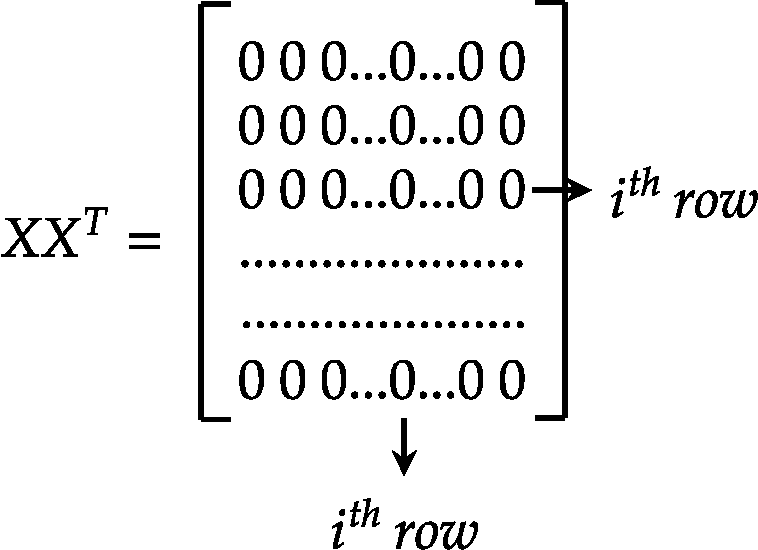
\includegraphics[height=4cm,width=6cm]{diagram-20210823(3)-crop}
		\end{figure}
		Since this matrix is diagonal, its eigenvalues are $a^{2}, 0,0 \ldots \ldots 0 .$ Hence, the number of non zero eigenvalues of the matrix $X X^{T}$ is 1 .\\\\
		So the correct answer is \textbf{Option (C)}
	\end{answer}
	\item The eigenvalues of a Hermitian matrix are all
	{\exyear{GATE 2018}}
	\begin{tasks}(4)
		\task[\textbf{A.}]  Real
		\task[\textbf{B.}] Imaginary
		\task[\textbf{C.}] Of modulus one
		\task[\textbf{D.}] Real and positive
	\end{tasks}
	\begin{answer}
		Eigenvalue of Hermitian matrix must be real.\\\\
		So the correct answer is \textbf{Option (A)}
	\end{answer}
	\item During a rotation, vectors along the axis of rotation remain unchanged. For the rotation matrix $\left(\begin{array}{ccc}0 & 1 & 0 \\ 0 & 0 & -1 \\ -1 & 0 & 0\end{array}\right)$, the vector along the axis of rotation is
	{\exyear{GATE 2019}}
	\begin{tasks}(2)
		\task[\textbf{A.}] $\frac{1}{3}(2 \hat{i}-\hat{j}+2 \hat{k})$
		\task[\textbf{B.}]  $\frac{1}{\sqrt{3}}(\hat{i}+\hat{j}-\hat{k})$
		\task[\textbf{C.}] $\frac{1}{\sqrt{3}}(\hat{i}-\hat{j}-\hat{k})$
		\task[\textbf{D.}] $\frac{1}{3}(2 \hat{i}+2 \hat{j}-\hat{k})$
	\end{tasks}
	\begin{answer}
		So the correct answer is \textbf{Option (B)}
	\end{answer}
\end{enumerate}
\colorlet{ocre1}{ocre!70!}
\colorlet{ocrel}{ocre!30!}
\setlength\arrayrulewidth{1pt}
\begin{table}[H]
	\centering
	\arrayrulecolor{ocre}
	\begin{tabular}{|p{1.5cm}|p{1.5cm}||p{1.5cm}|p{1.5cm}|}
		\hline
		\multicolumn{4}{|c|}{\textbf{Answer key}}\\\hline\hline
		\rowcolor{ocrel}Q.No.&Answer&Q.No.&Answer\\\hline
		1&\textbf{C} &2&\textbf{C}\\\hline 
		3&\textbf{D} &4&\textbf{C} \\\hline
		5&\textbf{B} &6&\textbf{5} \\\hline
		7&\textbf{D}&8&\textbf{C}\\\hline
		9&\textbf{A}&10&\textbf{B}\\\hline
		
	\end{tabular}
\end{table}